
\subsection{Using the Frobenius eigenvalue of $P(s)$}


In walking towards the end-goal of proving the Central Limit
Theorem for $M_n$ and Markov sources, a major step is finding
an expression that fits $V_n$ well enough. The candidate we
saw previously which came from~\cite{leckey_limit_2015} was 
only defined for Markov sources of order 1 and was not proved
to be a fitting candidate. Therefore, I was tasked to investigate
another expression, which appeared in the analysis of 
P. Jacquet and my supervisor's old paper~\cite{jacquet_average_2001}.
What I achieved here is to find several expressions of 
this variance candidate and run them against my simulations - eventually
finding out what seems to be the right candidate for the variance.

First, some definitions in order to introduce this candidate, and 
compute the exact expressions needed for simulation:

\begin{df}
    We define the matrix $P(s)$ from the probability matrix $P$ of a 
    Markov source as:
    \centers{$\forall s\in\mathbb{C} 
             \qquad P(s) = ({p_{i j}}^{-s})_{(i,j)\in{\{1,\dots,V\}}^2} $}
    \label{def:ps}
\end{df}

\begin{df}
    For $s\in\mathbb{C}$, the \emph{Frobenius eigenvalue} of $P(s)$ is the highest 
    eigenvalue of $P(s)$ in absolute value. It is denoted $\lambda(s)$.
    \label{def:frob}
\end{df}

\noindent
Ignoring the difficult steps it took to obtain it in~\cite{jacquet_average_2001},
this is the variance expression:

\encadre{$ {V_n}^{(2)} =  \left( \ddot{\lambda}(-1) - { \dot{\lambda}(-1) }^2 \right) \f{n}{\ln^2 n} $}

\noindent Let's compute $\ddot{\lambda}(-1)$ with a Markov chain of order 1.
In~\cite{jacquet_average_2001},
\centers
    {$ \ddot{\lambda}(-1) = \pi \ddot{P}(-1)\psi
                        + 2 \dot{\pi}(-1) \dot{P}(-1) \psi
                        - 2 \dot{\lambda}(-1) \dot{\pi}(-1) \psi $}

\noindent The vector $\pi(s)$, which coincides with the stationary
distribution $\pi$ for $s=-1$, is defined as the left-eigenvector of 
$\lambda(s)$ whose product with the right-eigenvector of $\lambda(s)$
makes $\lambda(s)$, which is written:
   
        \centers{ $ \left\{
            \begin{array}{rl} \pi(s) P(s)  &= \lambda(s) \pi(s) \\
                          P(s) \psi(s) &= \lambda(s) \psi(s) \\
                          \pi(s) \psi(s) &= \lambda(s) 
            \end{array}
                    \right. $}

\noindent
However, I failed at computing $\pi(s)$ using these expressions - they did not seem to allow me to 
directly compute $\dot{\pi}(s)$ as it seemed I needed one more to get rid of all the 
unknowns. So I took another approach and directly computed $\lambda(s)$ as the greatest 
eigenvalue of $P(s)$. Let $\chi$ be the characteristic polynomial of $P(s)$,
and $\Delta(s)$ its discrimant:

\centers{$ \chi = (X - {p_{0 0}}^{-s}) 
                  (X - {p_{1 1}}^{-s}) 
                    - (p_{0 1} \, p_{1 0})^{-s} $}

\begin{egalites}
& \Delta(s)
        & (\poo + \pii)^2 - 4[\pooii - \poiio] \\[1mm]
        && {p_{0 0}}^{-2s} 
                + {p_{1 1}}^{-s} - 2\pooii + 4\poiio
\end{egalites}

\noindent
 Informally, we have this expression for $\lambda(s)$ 
where we need to decide which sign is the correct one :
\encadre{$ \lambda(s) = \f{ \poo + \pii \pm \sqrt{\Delta(s)}}{2} $}

\noindent
Since $\Delta(-1) 
        = (p_{0 0} + p_{1 1})^2 
                        - 2 p_{0 0} p_{1 1} 
                        + 4 p_{0 1} p_{1 0}
        = (p_{0 0} + p_{1 1} - 2)^2 $, then $ \sqrt{ \Delta(-1) } = 2 - p_{0 0} - p_{1 1} = p_{0 1} + p_{1 0}$. 
Thus, picking the $+$ sign in the former expression, we verify that  
\centers{$ \lambda(-1) =  \f{ p_{0 0} + p_{1 1} + \sqrt{ \Delta(-1) } }
                                               {2} = 1 $}

\noindent Derivating
\centers
    {$ \dot{\lambda}(s) = \f12 \left( -\ln p_{0 0}\, \poo - \ln p_{1 1}\, \pii + \f{ \Delta'(s) }{ 2 \sqrt{\Delta(s)} } \right) $}

\noindent
with

\begin{calculs}
    &\Delta'(s) 
        &=& - 2 \ln p_{0 0}\, \poodeux - 2 \ln p_{1 1}\, \piideux \\
        &&&                + 2 \ln (p_{0 0} p_{1 1})\, \pooii 
                        - 4 \ln (p_{0 1} p_{1 0})\, \poiio
\end{calculs}

\noindent gives

\begin{calculs}
    &\Delta'(-1) 
        &=& - 2 \ln p_{0 0}\, {p_{0 0}}^2 - 2 \ln p_{1 1}\, {p_{1 1}}^2 \\
        &&& + 2 \ln (p_{0 0} p_{1 1})\, (p_{0 0} p_{1 1})
                        - 4 \ln (p_{0 1} p_{1 0})\, (p_{0 1} p_{1 0})
\end{calculs}

\noindent
Numerically, we verified that $ \dot{\lambda}(-1) = h $. Derivating again yields

\begin{calculs}
    &\ddot{\lambda}(s) 
        &=& \f12 \Bigg( \ln^2 p_{0 0} \poo + \ln^2 p_{1 1} \pii \\
        &&&  \qquad \quad         + \f{ \Delta''(s) \sqrt{\Delta(s)} - \Delta'(s) \cdot \tf{\Delta'(s)}
                                                                            {2\sqrt{\Delta(s)}} }
                        {2\Delta(s)} \Bigg)
\end{calculs}

\noindent with

\begin{calculs}
    &\Delta''(s) 
            &=& 4 \ln^2 p_{0 0}\, \poodeux + 4 \ln^2 p_{1 1}\, \piideux \\
            &&&         - 2 \ln^2 (p_{0 0} p_{1 1})\, \pooii
                     + 4 \ln^2 (p_{0 1} p_{1 0})\, \poiio
\end{calculs}

\noindent
Finally,

\begin{calculs}
    &\ddot{\lambda}(-1) 
        &=& \f12 \Bigg( \ln^2 p_{0 0}\, p_{0 0} + \ln^2 p_{1 1}\, p_{1 1} \\
        &&& \qquad\quad + \f{ \Delta''(-1) \sqrt{\Delta(-1)} - \tf { {\Delta'(-1)}^2 }
                {2\sqrt{\Delta(-1)}} } {2\Delta(-1)} \Bigg)
\end{calculs}

The simulations using this coefficient for the variance are quite good. It also seems that 
this formula for the variance is equivalent to the one used in the unpublished paper 
\emph{Probabilistic Analysis of Lempel-Ziv Parsing for Markov Sources} by Leckey, 
Wormald and Neininger, but our two ways of deriving it differs. Numerical instability
might account for the tiny differences found for high $n$ values ($10^7$), although
this hasn't been verified. 

\centers{
      \begin{figure}
        \centering
        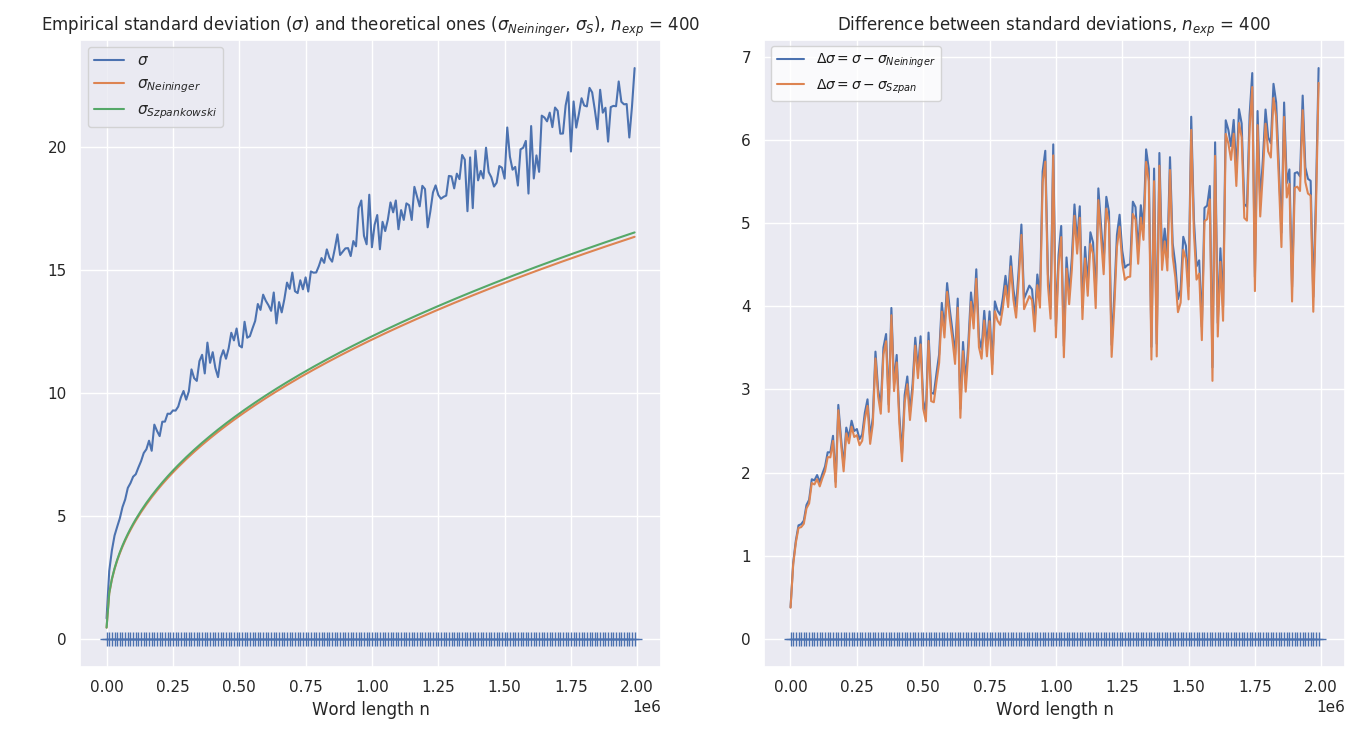
\includegraphics[width = 7.5cm,
        				    trim = 0 0 16.5cm 1.0cm,
                                clip=true]{./figs/eig_fig1.png}	
        \caption{Behavior of theoretical and standard deviations\\
                    $n_{\text{exp}} = 400$}
      \end{figure}
	}

\centers{
      \begin{figure}
        \centering
        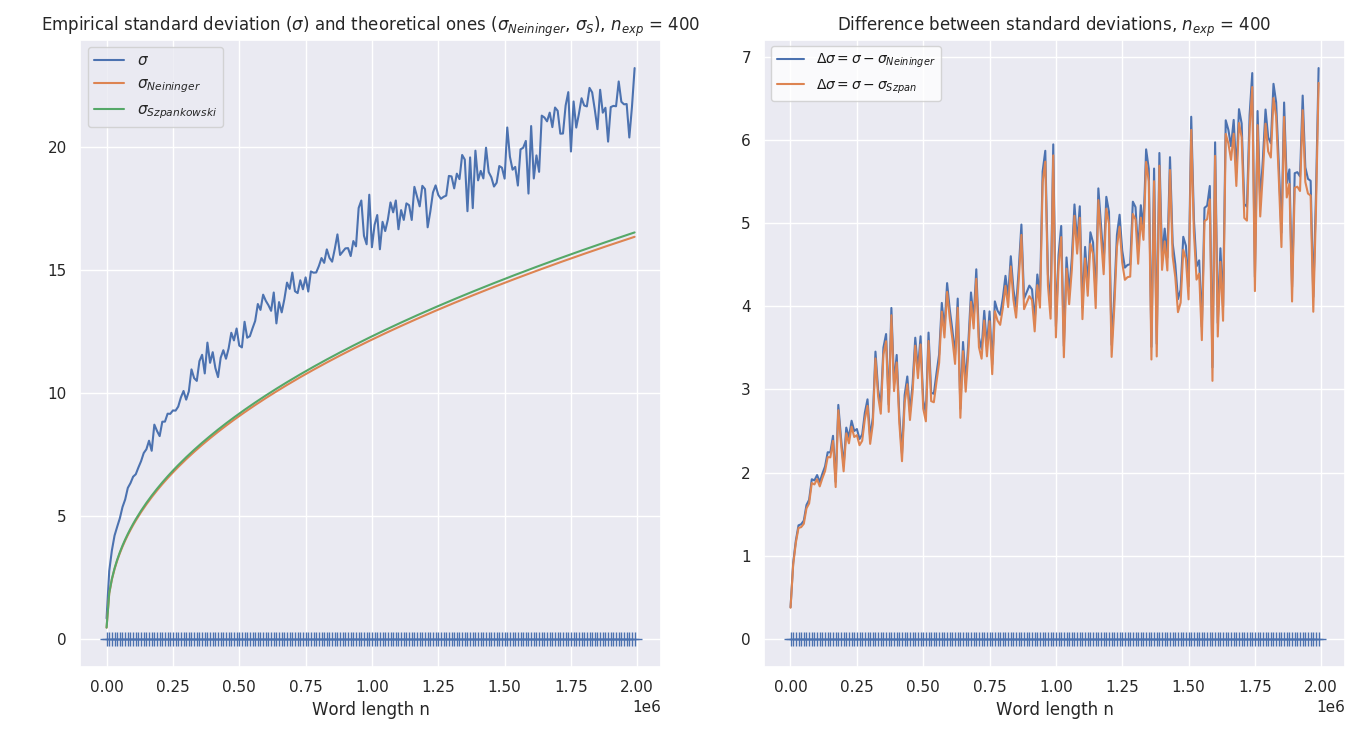
\includegraphics[width = 7.5cm,
        				    trim = 18.5cm 0 0 1.0cm,
                                clip=true]{./figs/eig_fig1.png}
        \captionsetup{justification=centering}
        \caption{Difference between empirical and theoretical standard deviations ($\sqrt{V_n}$)\\
                    $n_{\text{exp}} = 400$}
	\end{figure} 
	}

\pagebreak
Now, for some distributions of very long words that were normalized using 
our theoretical standard deviations, and empirical means. The blue plot is 
a gaussian fit for the simulation results, which also appear as a blue histogram.
The two sets of figures are identical but obtained using different expressions.

\centers{
      \begin{figure}[H]
        \centering
        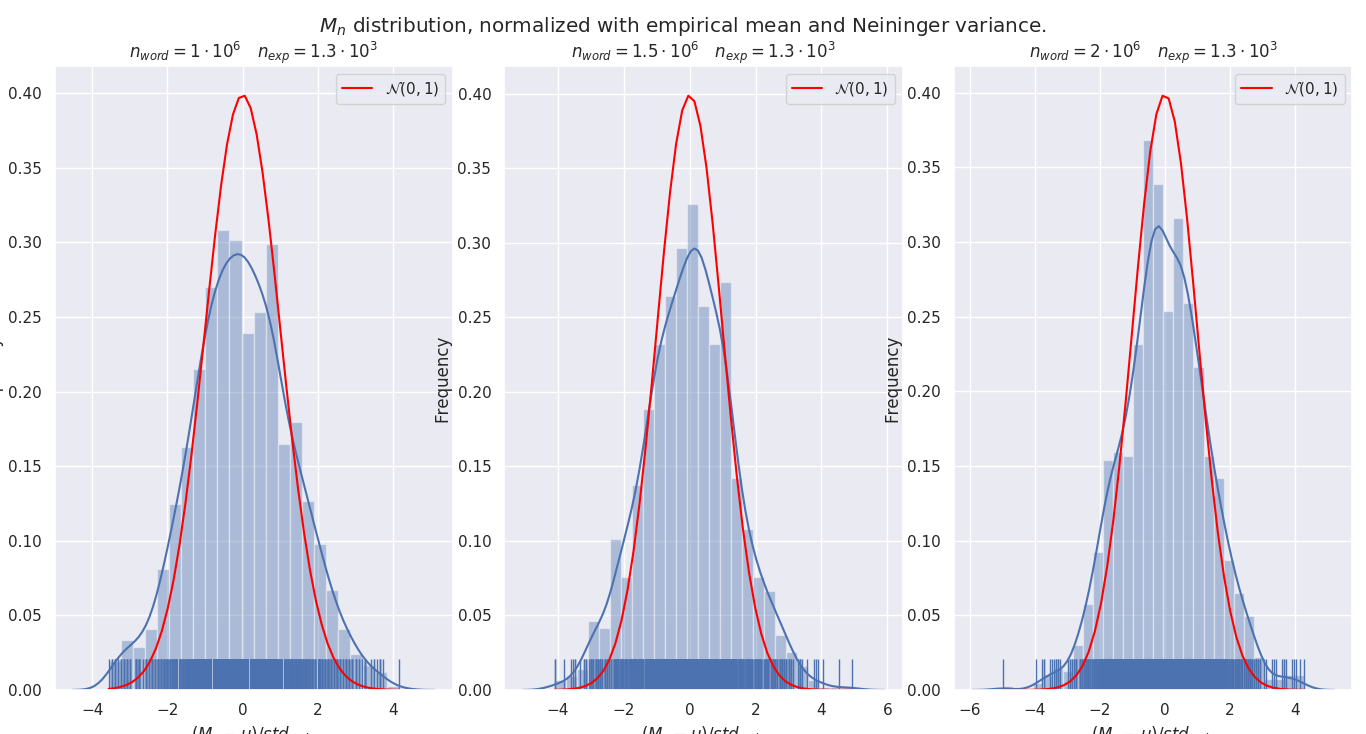
\includegraphics[width = \linewidth,
        				    trim = 0 0.5cm 0 1cm,
                                clip=true]{./figs/eig_fig3.png}	
                                \caption{Distribution of $M_n$ normalized with empirical mean and ${V_n}^{(1)}$ variance}
     \end{figure}
}

\centers{
      \begin{figure}
        \centering
        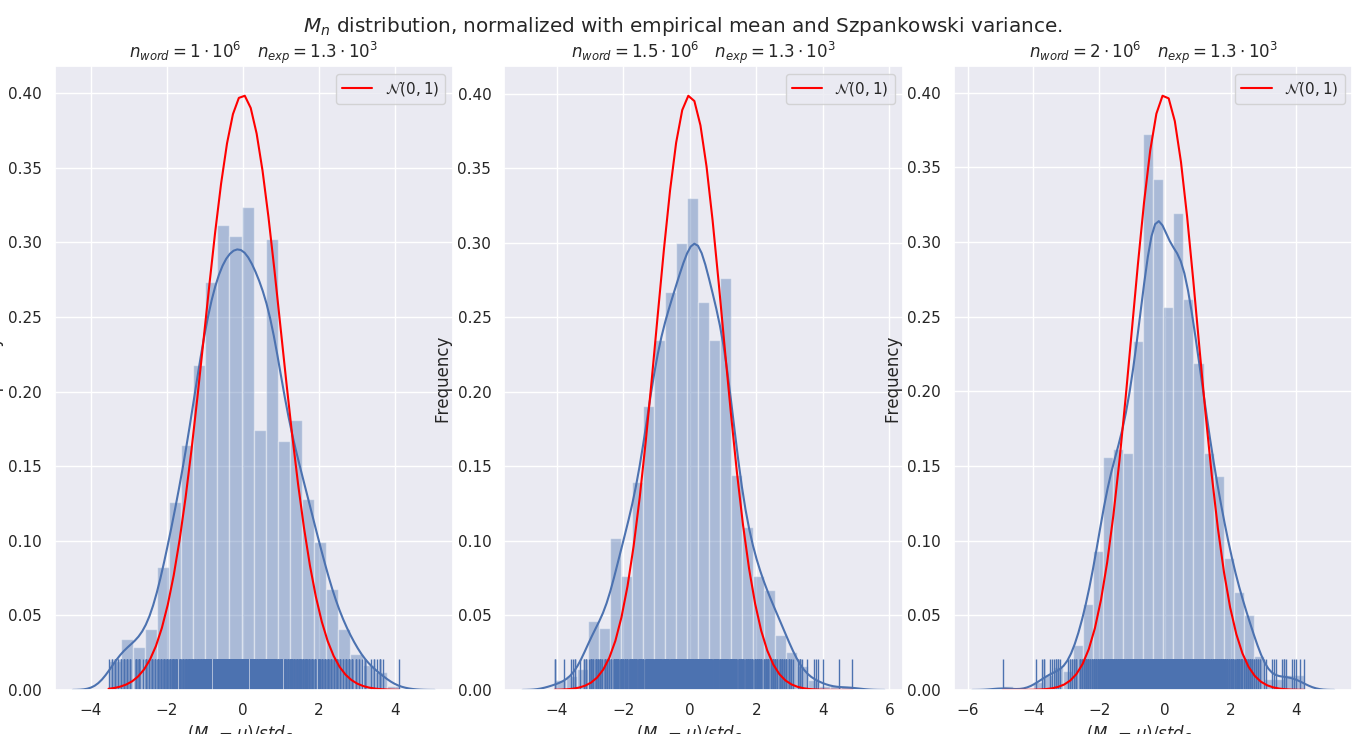
\includegraphics[width = \linewidth,
        				    trim = 0 0.5cm 0 1cm,
                                clip=true]{./figs/eig_fig2.png}	
        \caption{Distribution of $M_n$ normalized with empirical mean and ${V_n}^{(2)}$ variance}
      \end{figure}
} 


\section{Conclusion}
Similar results were obtained for a variety of randomly generated Markov sources,
which seem to indicate that this formula for the variance could be proven theoretically
correct. 

\begin{remarque}
\noindent \textbf{Limits of this work}


The figures suffer from imprecision over the computation of the empirical 
variance : this is due to the difficulties encountered in computing large amounts
of long words (of size over $10^6$). The figure in appendix \ref{app:much_longer} is 
an example of this limitation : with only 100 experiments, the empirical variance 
varies a lot. Possible ideas of improvement might come from parallelization,
rewriting functions in a computationnal language such as Julia, or using/devising a datastructure
specific to the task of building very long words.

Another problem is that the space of random Markov chains (here: stochastic matrices
of size 2) is not sampled thoroughly. Sampling a small number of Markov chains uniformly
according to their entropy might be interesting as a representation of the space,
 because otherwise it would be hard to sample a large number of stochastic matrices
due to the necessity of computing large words for each of them.

Finally, the difference between empirical $V_n$ and our expression seems to be growing
very slowly with $n$. This might be a term that is negligible (\textit{i.e.} of 
order lower than $\tf{n}{\log_2^2(n)}$), or a small detail in the formula of $V_n$. 
For example, the natural base logarithm (in $\tf{n}{\ln^2(n)}$) in the eigenvalue expression works slightly
better than the one in base 2 (in $\tf{n}{\log_2^2(n)}$), with the inverse situation happening for the first 
expression (${V_n}^{(1)}$). Anyway, the figures obtained seem to 
indicate that we are close to the exact solution.

\end{remarque}


The code for these experiments, with detailed procedures for reproducibility,
is hosted on GitHub in one of my \href{github.com/gliboc/lz-compression}{public repositories}.
Finally, another (probably bad) way of computing $\lambda(s)$ is in appendix \ref{app:comp_lam1}
for curiosity.



 
% \noindent First term is
% \centers
%     { $\pi_0 \, p_{0 0} \, \log^2 (p_{0 0}) 
%         + \pi_1 \, p_{1 0} \, \log^2 (p_{1 0}) 
%         + \pi_0 \, p_{0 1} \, \log^2 (p_{0 1}) 
%         + \pi_1 \, p_{1 1} \, \log^2 (p_{1 1})  $}

% \noindent The second is
% \centers
%     { $ - 2 \pac{
%             \dot{\pi}_0(-1) p_{0 0} \log (p_{0 0})    
%             + \dot{\pi}_1(-1) p_{1 0} \log (p_{1 0}) 
%             + \dot{\pi}_0(-1) p_{0 1} \log (p_{0 1})
%             + \dot{\pi}_1(-1) p_{1 1} \log (p_{1 1})
%         }   
%     $}

% \noindent The third is
% \centers{
%     $ - 2 \dot{\lambda}(-1) \pac{
%         \dot{\pi}_0(-1) 
%         + \dot{\pi}_1(-1)
%     }$
% }

% \noindent We 
%         have to compute $\dot{\pi}(-1)$. With 
%             $\pi(s) = (\pi_0(s), \, \pi_1(s))$, and since

% \centers{$\pi(s) P(s) = \lambda(s) \pi(s)$}

% \leftcenters
%     {then we have}
%     {$ \left\{
%         \begin{aligned}
%             {p_{0 0}}^{-s} \pi_0(s) + {p_{0 1}}^{-s} \pi_1(s) &= \lambda(s) \pi_0(s) \\
%             {p_{1 0}}^{-s} \pi_0(s) + {p_{1 1}}^{-s} \pi_1(s) &= \lambda(s) \pi_1(s) \\
%         \end{aligned}
%         \right.
%      $}

% which I'm not sure how to solve formally.
% \noindent
% solving for $\pi_0(s)$ and $\pi_1(s)$, 
% assuming $ p_{0 0} p_{1 1} \neq p_{0 1} p_{1 0} $ :

% \centers{$ \pi_0(s) = \lambda(s) \f{ \overbrace{{p_{1 1}}^{-s} - {p_{0 1}}^{-s}}^{g_0(s)} }
%                                    { \underbrace{{ (p_{0 0} p_{1 1}) }^{-s} 
%                                         - { (p_{0 1} p_{1 0}) }^{-s}}_{\delta(s)} }
%             \qquad 
%             \text{and}
%             \qquad
%        \pi_1(s) = \lambda(s) \f{ \overbrace{{p_{0 0}}^{-s} - {p_{1 0}}^{-s}}^{g_1(s)} }
%                                    { { (p_{0 0} p_{1 1}) }^{-s} 
%                                         - { (p_{0 1} p_{1 0}) }^{-s} }$}


% \leftcenters
%     {hence for $i\in\{0,1\}$}
%     {$ \dot{\pi}_i(s) = \dot{\lambda}(s) \f{g_i(s)}{\delta(s)}
%                         + \lambda(s) \f{{g_i}'(s)\delta(s) - g_i(s)\delta'(s)}
%                                         {\delta^2(s)}$}

% \leftcenters
%     {so}
%     {$ \dot{\pi}_i(-1) = h \f{g_i(-1)}{\delta(-1)}
%                         + \f{{g_i}'(-1) \delta(-1) - g_i(-1) \delta'(-1) }
%                             {\delta^2(-1)} $}

% \begin{egalites}
%     with & \delta(-1) 
%             & p_{0 0} p_{1 1} - p_{0 1} p_{1 0} \\[3mm]
%          &g_0(-1) 
%             & p_{1 1} - p_{0 1} \\[3mm]
%         &{g_0}'(-1)
%             & -\ln (p_{1 1}) p_{1 1} + \ln (p_{0 1}) p_{0 1} \\[3mm]
%         &g_1(-1)
%             & p_{0 0} - p_{1 0} \\[3mm]
%         &{g_1}'(-1) 
%             & -\ln (p_{0 0}) p_{0 0} + \ln (p_{1 0}) p_{1 0} 
% \end{egalites}


% \leftcenters
%     {where}
%     {  $\left\{
%         \begin{minipage}{0.6\textwidth}
%        $ {g_0}'(s) = - \ln(p_{1 1}) {p_{1 1}}^{-s}
%                  + \ln(p_{0 1}) {p_{0 1}}^{-s}$ \\[3mm]
%         $\delta'(s) = - \ln( p_{0 0} p_{1 1}) { (p_{0 0} p_{1 1}) }^{-s}
%                         +  \ln ( p_{0 1} p_{1 0} ) { (p_{0 1} p_{1 0}) }^{-s} $
%         \end{minipage}
%         \right.$ }



% \noindent
% Now taking $s=-1$ and re-arranging in a linear system of unknown $\dot{\pi}_0(-1)$ and $\dot{\pi}_1(-1)$ :
% \centers
%     {$ \left\{
%         \begin{aligned}
%             \dot{\pi}_0(-1) (p_{0 0} - \lambda)
%             + \dot{\pi}_1(-1) p_{0 1}
%                 &= \dot{\lambda}(-1) \pi_0
%                     +   \ln p_{0 0} \cdot p_{0 0} \pi_0
%                     +   \ln p_{0 1} \cdot p_{0 1} \pi_1 \\
%             \dot{\pi}_0(-1) p_{1 0}
%             + \dot{\pi}_1(-1) (p_{1 1} - \lambda)
%                 &= \dot{\lambda}(-1) \pi_1
%                     +  \ln p_{1 0} \cdot p_{1 0} \pi_0 
%                     +  \ln p_{1 1} \cdot p_{1 1} \pi_1
%         \end{aligned}
%         \right.
%      $}

% \noindent since
% $\dot{\lambda}(-1) = h$ and,
% $\lambda(-1) = 1$ :

% \centers
%     {$ \left\{
%         \begin{aligned}
%             \dot{\pi}_0(-1) (p_{0 0} - 1)
%             + \dot{\pi}_1(-1) p_{0 1}
%                 &= h \pi_0
%                     +   \ln p_{0 0} \cdot p_{0 0} \pi_0
%                     +   \ln p_{0 1} \cdot p_{0 1} \pi_1 \\
%             \dot{\pi}_0(-1) p_{1 0}
%             + \dot{\pi}_1(-1) (p_{1 1} - 1)
%                 &= h \pi_1
%                     +  \ln p_{1 0} \cdot p_{1 0} \pi_0 
%                     +  \ln p_{1 1} \cdot p_{1 1} \pi_1
%         \end{aligned}
%         \right.
%      $}

% \begin{egalites}
% which is  &\lambda
%         &\f{ (p_{0 0} + p_{1 1}) 
%            + \sqrt{ (p_{0 0} + p_{1 1})^2 - 4 (p_{0 0} p_{1 1} - p_{1 0} p_{0 1}) }}
%            {2}\\[3mm]
%         &&\f{ (p_{0 0} + p_{1 1}) 
%            + \sqrt{ (p_{0 0} - p_{1 1})^2 + 4 p_{1 0} p_{0 1} }}
%            {2}   
% \end{egalites}





